\label{sec:results_part2}
We devote this section to deliver the classification performance of our proposed pipeline. Details can be found in \texttt{my\_notebook.ipynb}.
As described in \textbf{Sec. \ref{sec:part2_method}}, \textbf{Protocol A} is free of data leakage, but \textbf{Protocol B} is not totally free of it, and varies differently depending on each fold.
This does not affect our ablation studies in \textbf{Sec. \ref{sec:ablation_part1}}, because the data leakage is attributed to our newly introduced CNN–based feature extractors and feature compressor.

\begin{table}[H]
    \centering
    \caption{\textbf{Protocol B} class–wise performance metrics across models.}
    \label{tab:cv_classwise_part2}

    \begin{subtable}[t]{0.48\textwidth}
        \centering
        \caption{KNN}
        \label{tab:cv_knn_part2}
        \begin{tabular}{cccc}
            \toprule
            Class & Precision & Recall & F1 Score \\
            \midrule
            NORM (0) & 81.8 & 61.5 & 70.2 \\
            MI   (1) & 39.0 & 43.9 & 41.3 \\
            STTC (2) & 40.3 & 49.1 & 44.2 \\
            HYP  (3) & 18.4 & 50.4 & 26.9 \\
            CD   (4) & 50.9 & 64.9 & 56.9 \\
            \bottomrule
        \end{tabular}
    \end{subtable}
    \hfill
    \begin{subtable}[t]{0.48\textwidth}
        \centering
        \caption{Random Forest}
        \label{tab:cv_rf_part2}
        \begin{tabular}{cccc}
            \toprule
            Class & Precision & Recall & F1 Score \\
            \midrule
            NORM (0) & 82.6 & 80.8 & 81.7 \\
            MI   (1) & 51.4 & 50.8 & 51.1 \\
            STTC (2) & 51.8 & 51.4 & 51.5 \\
            HYP  (3) & 30.3 & 38.4 & 33.7 \\
            CD   (4) & 64.3 & 68.2 & 66.1 \\
            \bottomrule
        \end{tabular}
    \end{subtable}

    \bigskip

    \begin{subtable}[t]{0.48\textwidth}
        \centering
        \caption{Histogram–based Gradient Boosting}
        \label{tab:cv_gb_part2}
        \begin{tabular}{cccc}
            \toprule
            Class & Precision & Recall & F1 Score \\
            \midrule
            NORM (0) & 87.2 & 73.1 & 79.5 \\
            MI   (1) & 48.2 & 53.8 & 50.8 \\
            STTC (2) & 50.8 & 59.6 & 54.8 \\
            HYP  (3) & 26.6 & 51.9 & 35.1 \\
            CD   (4) & 61.5 & 70.2 & 65.5 \\
            \bottomrule
        \end{tabular}
    \end{subtable}
    \hfill
    \begin{subtable}[t]{0.48\textwidth}
        \centering
        \caption{AdaBoost}
        \label{tab:cv_ada_part2}
        \begin{tabular}{cccc}
            \toprule
            Class & Precision & Recall & F1 Score \\
            \midrule
            NORM (0) & 82.7 & 64.1 & 72.2 \\
            MI   (1) & 37.4 & 39.7 & 38.4 \\
            STTC (2) & 37.2 & 41.8 & 39.1 \\
            HYP  (3) & 14.1 & 47.2 & 21.7 \\
            CD   (4) & 46.4 & 54.0 & 49.6 \\
            \bottomrule
        \end{tabular}
    \end{subtable}

    \bigskip

    \begin{subtable}[t]{0.48\textwidth}
        \centering
        \caption{CatBoost}
        \label{tab:cv_cat_part2}
        \begin{tabular}{cccc}
            \toprule
            Class & Precision & Recall & F1 Score \\
            \midrule
            NORM (0) & 86.5 & 75.0 & 80.3 \\
            MI   (1) & 49.6 & 54.3 & 51.8 \\
            STTC (2) & 52.2 & 60.2 & 55.9 \\
            HYP  (3) & 28.9 & 52.8 & 37.3 \\
            CD   (4) & 64.1 & 69.9 & 66.8 \\
            \bottomrule
        \end{tabular}
    \end{subtable}
    \hfill
    \begin{subtable}[t]{0.48\textwidth}
        \centering
        \caption{XGBoost}
        \label{tab:cv_xgb_part2}
        \begin{tabular}{cccc}
            \toprule
            Class & Precision & Recall & F1 Score \\
            \midrule
            NORM (0) & 85.6 & 74.7 & 79.7 \\
            MI   (1) & 48.4 & 53.4 & 50.8 \\
            STTC (2) & 52.2 & 60.0 & 55.7 \\
            HYP  (3) & 28.4 & 46.6 & 35.2 \\
            CD   (4) & 62.5 & 69.6 & 65.8 \\
            \bottomrule
        \end{tabular}
    \end{subtable}
\end{table}

We remark that, \textbf{Tab. \ref{tab:single_model_wise_part2}} and \textbf{Tab. \ref{tab:cv_classwise_part2}} do not totally correctly reflect models' performance on 10–fold CV.
As we mentioned earlier, the extractors were trained on a 80\% train data. Meanwhile, in \textbf{Protocol B}, we split in 10 different folds to evaluate the models' performance.
Therefore, in each 10\% test of each fold, there may contain some leak training data. On the other hand, this also implies there are some unseen samples in the train set.
Together, we believe this may alleviate the impact of data leakage on \textbf{Protocol B}.
However, as an excuse, owing to resources constraints, we are unable to re–train \texttt{CNN–based} extractor and \texttt{encoder} on all 10 folds.

\begin{table}[H]
    \centering
    \caption{\textbf{Protocol B} Performance metrics across all models.}
    \label{tab:single_model_wise_part2}
    \begin{tabular}{ccccccc}
        \toprule
        Metrics & \texttt{XGBoost} & \texttt{RF} & \texttt{CatBoost} & \texttt{AdaBoost} & \texttt{GBoost} & \texttt{KNN} \\
        \midrule
        Precision & 55.4 & 56.1 & 56.3 & 43.6 & 54.8 & 46.1 \\
        Recall & 60.8 & 57.9 & 62.5 & 49.3 & 61.7 & 53.9 \\
        F1 Score & 57.5 & 56.8 & 58.4 & 44.2 & 57.1 & 47.9 \\
        Accuracy & $67.7$ & $69.1$ & $68.4$ & $55.4$ & $67.1$ & $56.9$ \\
        \midrule
        \midrule
        Time (s) & 9.2 & 17.4 & 57.2 & 33.0 & 52.8 & 0.9 \\
        \bottomrule
    \end{tabular}
\end{table}

Considering the tables above, our pipeline improves every classifier over the reproduction in \textbf{Tab. \ref{tab:single_model_wise}}.
Macro F1 rises by $16.6$–$18.1$ points for the four ensembles and by $22.5$ for \texttt{KNN} ($25.4 \rightarrow 47.9$), the largest gain of all.
The ensembles lie within $1.6$ F1 of one another ($56.8$–$58.4$): \texttt{CatBoost} attains the highest F1 and \texttt{RF} the highest accuracy ($69.1\%$).
Fitting the classifiers is also $2.6$–$9.8\times$ faster, e.g. $322.2 \rightarrow 33.0$\,s for \texttt{AdaBoost}, although this excludes the feature extractors.

Class–wise (\textbf{Tab. \ref{tab:cv_classwise_part2}} against \textbf{Tab. \ref{tab:cv_classwise}}), the largest average F1 gains are on CD ($+31.6$) and STTC ($+26.2$).
HYP barely moves: its F1 stays at $21.7$–$37.3$ and falls for three of the six models, while its precision ($14.1$–$30.3$) is far below its recall ($38.4$–$52.8$), i.e. every model over–predicts the rarest class.

The held–out split suggests the leakage in \textbf{Protocol B} is modest.
On the $3{,}249$ unseen records of \textbf{Fig. \ref{fig:part2_confusion}}, the ensembles reach $64.9$–$66.8\%$ accuracy, $1.0$–$2.3$ points below their 10–fold scores, whereas in \textbf{Part 1} this gap stayed within $0.5$ for the same models.
In \textbf{Fig. \ref{fig:part2_roc}}, their class–wise AUCs rise to $0.81$–$0.90$ from $0.65$–$0.88$ in \textbf{Fig. \ref{fig:reproduced_roc}}, with MI the hardest class ($0.81$–$0.83$) and CD the easiest ($0.89$–$0.90$).

\begin{figure}[H]
    \centering
    \caption{\textbf{Protocol A} Confusion matrices of all classifiers.}
    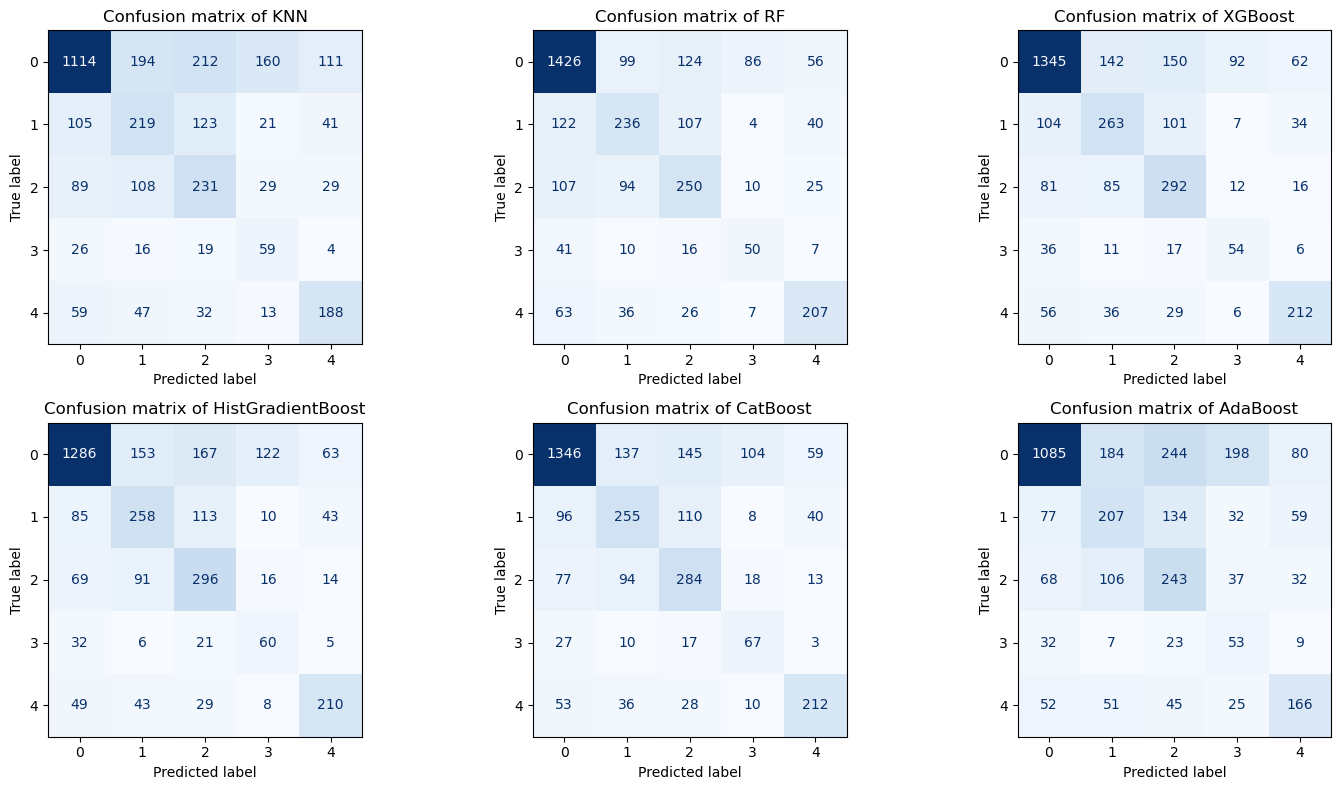
\includegraphics[width=\textwidth]{figures/part2/confusion_matrix.png}
    \label{fig:part2_confusion}
\end{figure}

\begin{figure}[H]
    \centering
    \caption{\textbf{Protocol A} ROC–AUC curves and scores across classifiers.}
    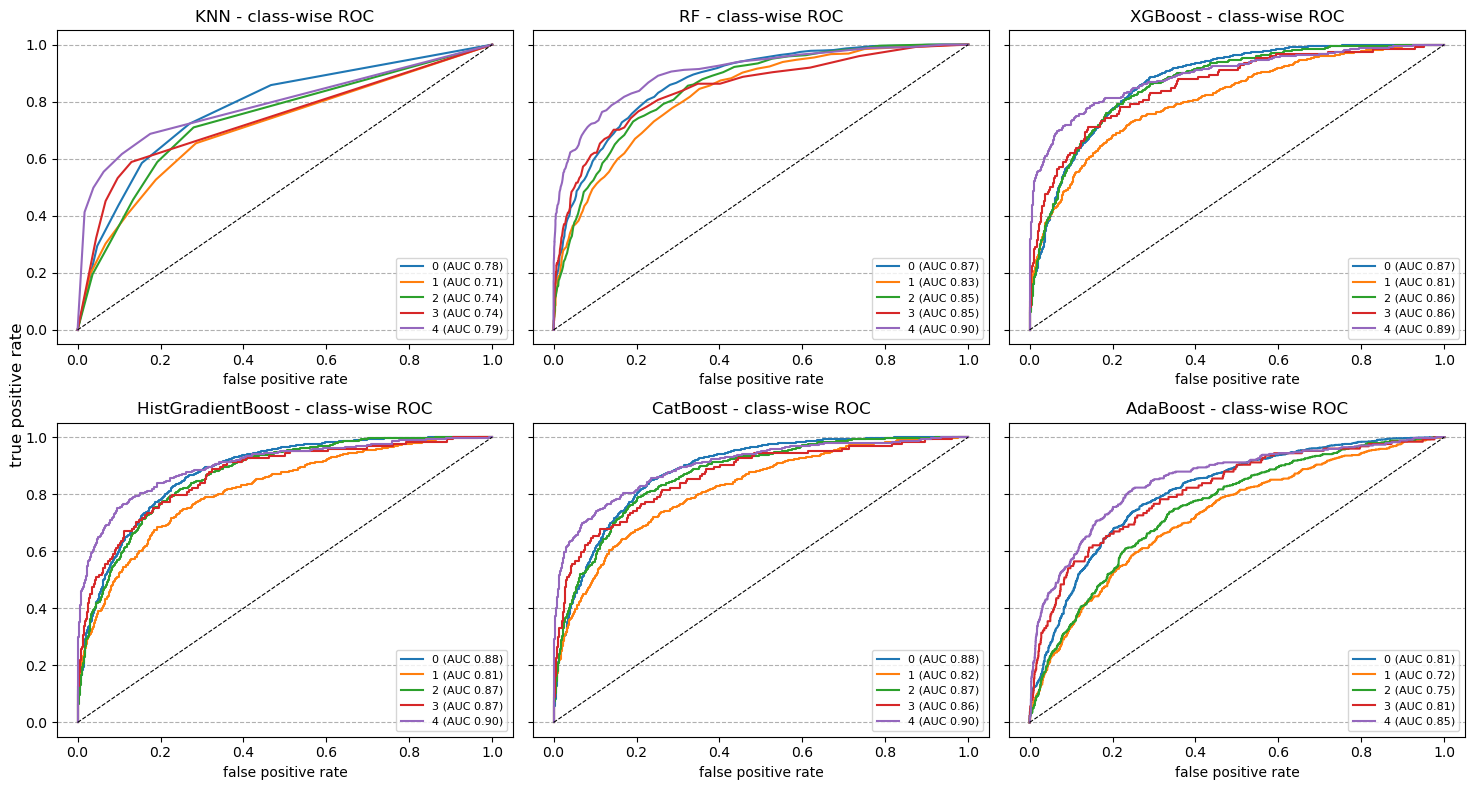
\includegraphics[width=\textwidth]{figures/part2/roc_curves.png}
    \label{fig:part2_roc}
\end{figure}